\section{Initial set of rectangles}

\begin{theorem}[Hall]
	The Markov and Lagrange spectra contain all the real numbers from some point, particularly,
	there exists a real $\mu$ such that
	\begin{equation*}
		[\mu; + \infty) \subset M \cap L.
	\end{equation*}
\end{theorem}

Hall proved the constant $\mu$ to be smaller than 7. In 1975 Freiman evaluated it:

\begin{theorem}[Freiman, 1975]
	For constants
	$ \mu = f \left( \overline{121313}2234 \underset{0}{4} 3211 \overline{313121} \right) $
	and \\
	$ \nu = f \left( \overline{323444}31313 \underset{0}{4} 313121133 \overline{313121} \right)$, having
	\begin{equation*}
		(\nu; \mu) \cap (\R \backslash L) = \emptyset,
		\quad
		[\mu; + \infty) \subset L \subset M.
	\end{equation*}
\end{theorem}

We present a set of rectangles
whose projections cover the segment from the Freiman's constant to $\sqrt{21}$.
All of them are good.
The reader is invited to find
the the algorithm of splitting these rectangles into subrectangles correctly in \cite{Freiman}.

\begin{figure}[H]
	\centering
	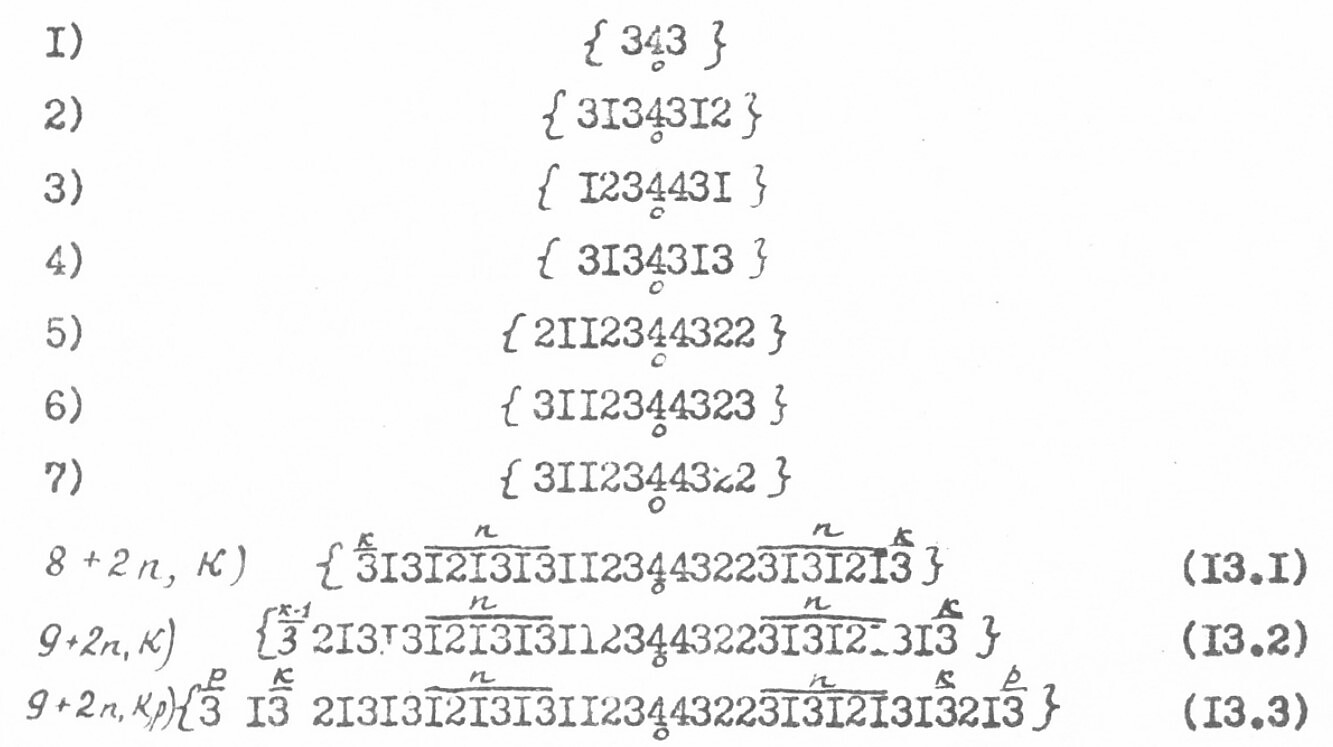
\includegraphics[width=0.8\textwidth]{initial-set}
	\caption{Initial set of rectangles.}
	\label{initial-set}
\end{figure}
